\documentclass[12pt, twoside, letterpaper]{report}
\usepackage[top=2cm,bottom=4cm,left=3cm,right=3cm,asymmetric]{geometry}

\usepackage{fancyhdr}
\pagestyle{fancy}
\fancyfoot[C]{}    
\fancyfoot[LE,RO]{\thepage}        
\fancyhead[RO]{\slshape \rightmark}
\fancyhead[LE]{\slshape\leftmark}      
\fancyhead[RE,LO]{}

\usepackage{color}   
\usepackage{hyperref}
\usepackage[utf8x]{inputenc}
\usepackage[italian]{babel}
\usepackage{amsmath, amsthm, amssymb, amsfonts}
\usepackage{blindtext}
\usepackage{dirtytalk}
\usepackage{cite}
\usepackage[breakable]{tcolorbox}
\usepackage{pdfpages}
\usepackage{enumitem}
\usepackage{caption}
\usepackage{subcaption}
\usepackage{graphicx}
\graphicspath{ {./img/} }
\newcommand{\img}[4] {
	\begin{figure}
		\centering
		\includegraphics[scale=#2]{#3}\\
		\caption{#1}
		\label{#4}
	\end{figure}
}

\title{Uso di reti neurali per la classificazione di dati in problemi di medicina legale}
\author{Mario Petruccelli \cr Università degli studi di Milano}
\date{A.A. 2019/2020}

\begin{document}

	\begin{titlepage}
		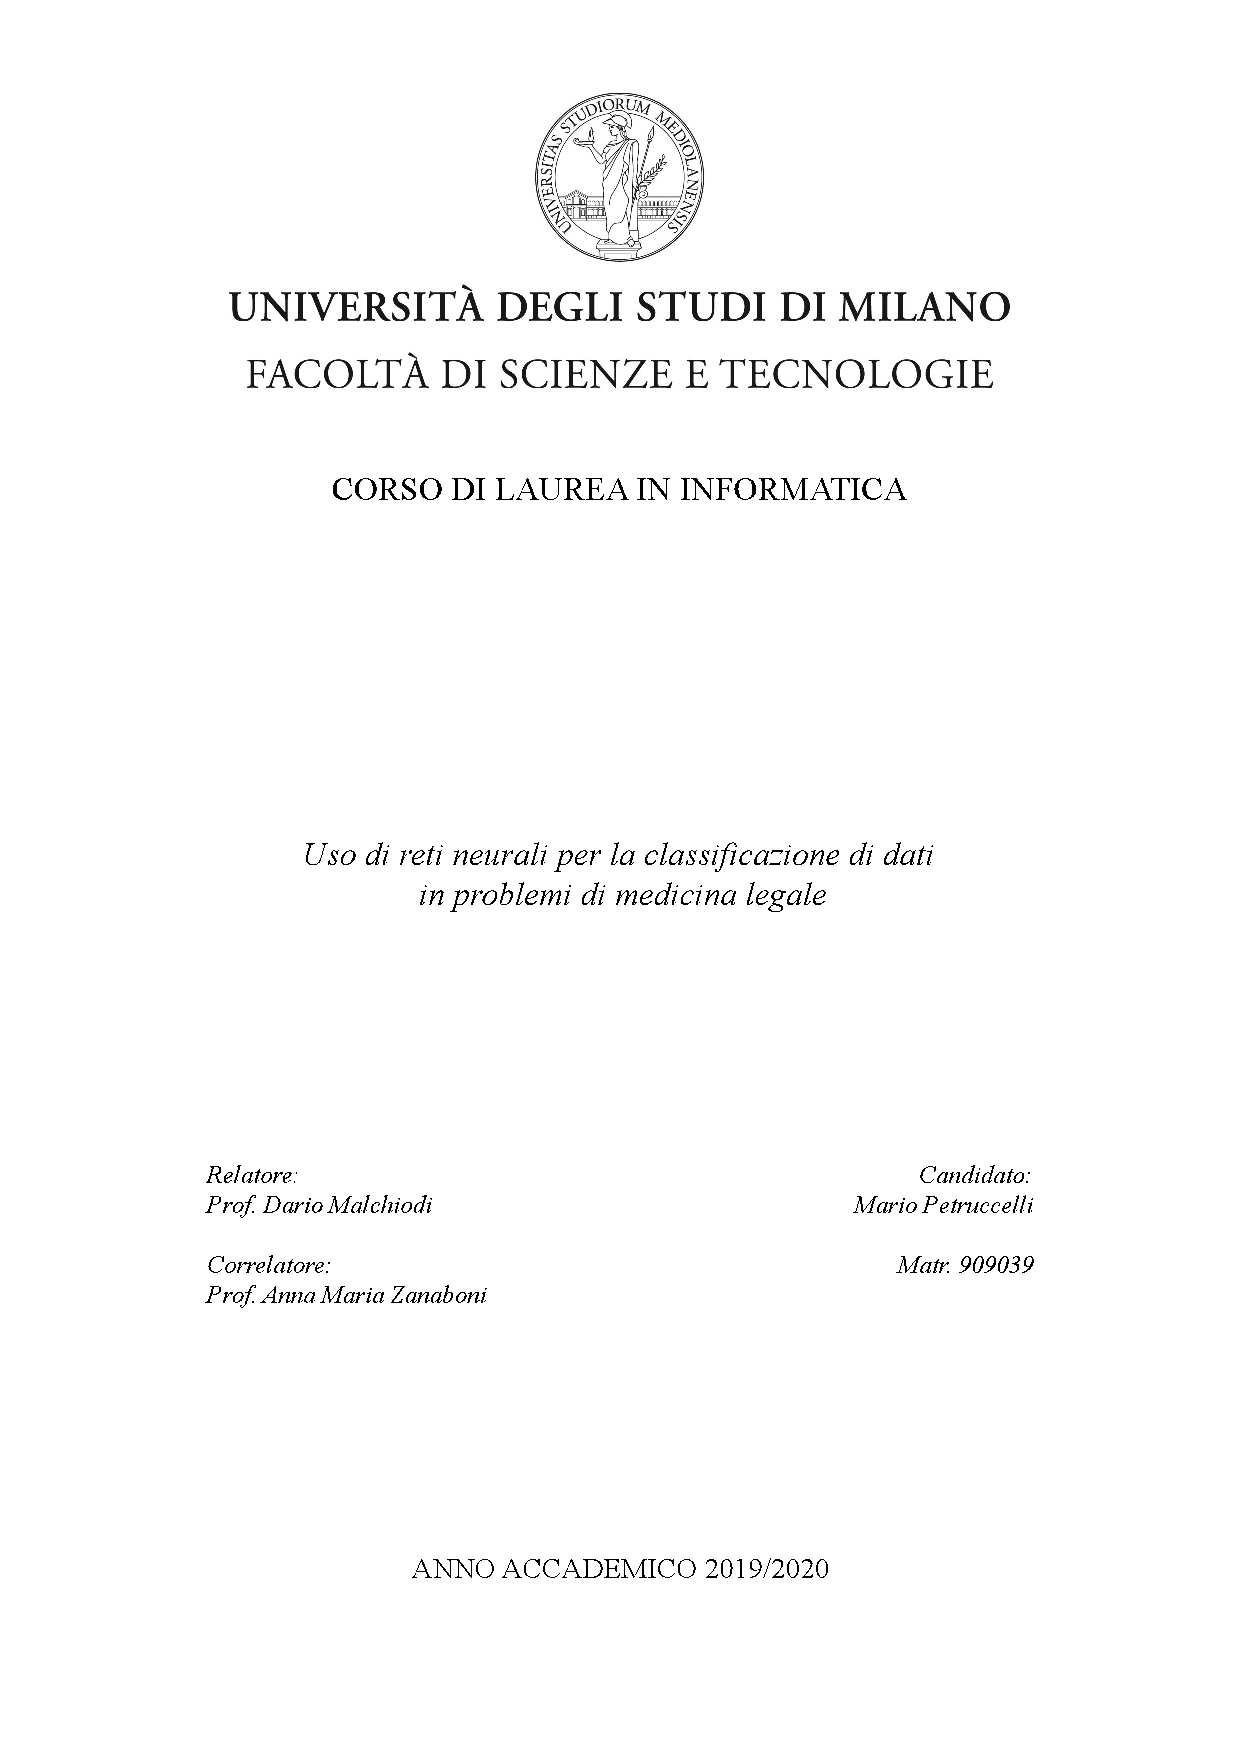
\includepdf{img/FRONTESPIZIO.pdf}
		\newpage
		\tableofcontents
		\thispagestyle{empty}
	\end{titlepage}

	\chapter*{Introduzione} \markboth{Introduzione}{}  \addcontentsline{toc}{chapter}{Introduzione}  \pagenumbering{arabic}
		Qua ci andrà l'introduzione

		\newpage		
	\chapter{Reti neurali}
		Le \textbf{reti neurali artificiali} sono un modello matematico molto importante del \textit{machine learning} che prende ispirazione dalle reti neurali biologiche presenti nel cervello animale. In questo capitolo vedremo le componenti e il funzionamento delle reti neurali artificiali, ma prima facciamo un'overview su cosa sia il machine learning.

		\section{Paradigma del machine learning}
			Il machine learning è una branca dell'intelligenza artificiale ed è una di quelle in più rapida espansione; negli ultimi decenni è diventato di uso comune in moltissime applicazioni che richiedono l'estrazione di informazioni dai dati. Lo scopo del machine learning è quello di riassumere tante istanze di un problema, che difficilmente sarebbero riconoscibili con l'uso tradizionale della programmazione \textit{(per esempio riconoscere la razza di un cane partendo da una foto)}.   
			
			Prendendo come esempio noi umani, molte delle nostre abilità vengono acquisite o raffinate dalla nostra esperienza, e così \textit{apprendiamo}. Immaginiamo di trovarci davanti un essere vivente che non abbiamo mai visto prima. Nonostante questo essere sia nuovo ai nostri occhi, sapremo riconoscere con molta probabilità se questo si tratti di un insetto, di un mammifero o di una pianta. Lo stesso concetto possiamo provare ad applicarlo alle macchine, ma come possono apprendere? 
			
			\subsection{Tipi di apprendimento} Il machine learning è diviso in diversi sottocampi in cui abbiamo più paradigmi di apprendimento. La principale distinzione che si può fare è la differenza tra l'apprendimento \textbf{supervisionato}, \textbf{non supervisionato} e \textbf{per rinforzo}. Per quanto riguarda ciò che vedremo nei prossimi capitoli, possiamo concentrarci solo sulla differenza tra l'apprendimento supervisionato e non supervisionato.
			
				\paragraph{Apprendimento supervisionato} Consideriamo di dover classificare tre specie di fiori leggermente diversi tra loro appartenenti alla stessa famiglia \textit{(esperimento che riprenderemo più avanti)}. Per imparare a riconoscerli, potremmo ricevere un insieme di dati \textit{(per esempio la larghezza dei petali, lunghezza del gambo, ecc...)} che descrivono i fiori e cercare di indovinare la specie. Una figura d'insegnante (\textit{teacher}) ci da una \textbf{risposta d'apprendimento} per ogni tentativo che facciamo di indovinare l'\textbf{etichetta}, ovvero la classe di cui fanno parte. Dopo questa fase di \textbf{allenamento}, dovremmo essere in grado di trovare un pattern tra i dati per etichettare nuovi fiori, questa volta privi di etichetta e non appartenenti all'insieme dato in precedenza. 
										
					In maniera più astratta, possiamo vedere questo come un processo di \textit{utilizzo dell'esperienza passata per acquisire competenza}. L'apprendimento supervisionato descrive uno scenario in cui dobbiamo utilizzare l'esperienza acquisita tramite il processo di apprendimento con un insieme di dati (\textbf{insieme di training}) per \textbf{predire} un'informazione mancante. La bontà di questo processo la si può testare con un altro insieme (\textbf{insieme di test}) calcolando l'errore in base a quante etichette vengono predette in modo corretto. 
				
				\paragraph{Apprendimento non supervisionato}  Nell'apprendimento non supervisionato non c'è distinzione tra i dati di training e di test. Vengono processati i dati con lo scopo di produrre una versione compressa, o un \say{riassunto} di essi. Il clustering, overro il raggruppamento dei dati in sottoinsiemi con caratteristiche simili è una delle pratiche più usate in questo campo.\\\\
				Il modello di cui ci occuperemo noi, ovvero le reti neurali artificiali, utilizzano un'apprendimento di tipo supervisionato.
				
				
		\section{Che cos'è una rete neurale?}
			Il cervello animale è un meccanismo in grado di apprendere grazie all'esperienza, ed è per questo che si è cercato di emularlo \textit{(in modo molto semplificato)} come modello di machine learning. Il nucleo di tale organo sono i \textbf{neuroni}, ed essi sono connessi tra di loro da delle \textbf{sinapsi} in modo da poter comunicare. Ebbene, anche il modello artificiale riprende questa forma. L'archetipo matematico di neurone è stato ideato da McCulloch e Pitts nell'articolo \textit{A logical calculus of the ideas immanent in nervous activity} del 1943. Lo descrivono come un modello contenente una soglia che ne determina lo stato di attivazione e una funzione non lineare detta \textbf{funzione di attivazione} che riceve uno o più input \textbf{pesati} e produce un unico output.
			
		\subsection{Componenti principali di una rete neurale} 
			\paragraph{Concetto di tempo} Prima di dare una definizione, introduciamo il concetto di tempo in una rete neurale. Ci si riferisce al tempo vigente come $(t)$, al passo successivo come $(t+1)$, al passo precedente come $(t-1)$, e così via. $t$ assume solo valori discreti.
			
			\paragraph{Rete neurale artificiale} Una rete neurale artificiale è formata da un insieme di \textbf{nodi} \textit{(neuroni)}, che elaborano le informazioni ricevute e trasmettono il risultato ai nodi successivi, e da \textbf{archi orientati pesati} \textit{(sinapsi)}. Più formalmente, una rete neurale è una tripla $(N,V, \omega)$ in cui:
			\begin{itemize}
				\item $N$ è l'insieme dei neuroni,
				\item $V = \{(i,j) | i,j \in N\}$ è l'insieme delle connessioni tra i neuroni $i$ e $j$, 
				\item $\omega: V \rightarrow \mathbb{R}$ è la funzione di peso, dove $\omega_{i,j}$ è il peso della connessione tra i neuroni $i$ e $j$.  
			\end{itemize}
			Un neurone elabora i dati che gli arrivano tramite le sue connessioni. Questo accade attraverso tre funzioni: funzione di \textbf{propagazione}, funzione di \textbf{attivazione} e funzione di \textbf{uscita}.
			
			\img{Struttura di un neurone \cite{kriesel}}{0.4}{neurone.png}{neurone} 
			
			 \paragraph{Funzione di propagazione} Dato un neurone $j$, la sua funzione di propagazione riceve gli output $o_{i_1}, \dots, o_{i_k}$ dei neuroni $i_1, \dots, i_k$ connessi a $j$ e i corrispettivi pesi $\omega_{i,j}$, restituendo un valore detto \textit{network input} net$_j$ che verrà poi processato dalla \textit{funzione di attivazione}. 
			 	
			 	Sia $I = \{i_1, i_2, \dots, i_k\}$ l'insieme dei neuroni connessi a $j$ tale che $I \neq \O, (\forall z \in \{1, \dots, k\} : \exists w_{i_z,j})$. Allora il network input di $j$ ($net_j$), è calcolato dalla funzione di propagazione $f_{prop}$ come segue: $$net_j = f_{prop}(o_{i_1}, \dots, o_{i_k},w_{i_1,j}, \dots, w_{i_k,j})$$
			 	La funzione di propagazione più usata è la \textbf{somma pesata}, ovvero la somma delle moltiplicazioni dell'output di ogni neurone $i$ per il corrispettivo peso $\omega_{i,j}$: $$net_j = \sum_{i \in I} o_i w_{i,j}$$
			 	
			 \paragraph{Stato di attivazione e valore di soglia} Ad ogni istante un neurone può essere \textit{attivo} o meno. Lo \textbf{stato di attivazione} \textit{(o attivazione)} è una reazione ai valori ricevuti in input, e il neurone viene attivato quando il \textit{network input} supera il \textbf{valore di soglia} di quel neurone. 
			 
			 Sia $j$ un neurone. L'ouput della funzione di attivazione di $j$ è un valore continuo, mentre lo stato di attivazione è un valore discreto. Il \textbf{valore di soglia} $\Theta_j$ è assegnato unicamente a $j$ e rappresenta il punto di massima pendenza della funzione di attivazione, oltre il quale si considera $j$ attivo.
			 
			 
			 \paragraph{Funzione di attivazione} Sia $j$ un neurone. La funzione di attivazione è così definita: $$a_j(t) = f_{act}(net_j(t), \Theta_j)\footnote{In alcune reti neurali ricorsive è presente come parametro della funzione anche il precedente stato di attivazione $a_j(t-1)$.}.$$ 
			 
			 	In funzione del \textit{network input} net$_j$ e dell valore di soglia $\Theta_j$ ricava un nuovo stato di attivazione $a_j(t)$
			 	A differenza di molte delle variabili definite prima, la funzione di attivazione viene definita \textit{globalmente} per ogni strato di neuroni. Esistono diverse funzioni di attivazione, alcune tra le più usate, come possiamo vedere in figura~\ref{fig:funzioni di attivazione} sono: 
			 	\begin{itemize}
			 		\item la funzione logistica: $f(x) = \frac{1}{1+e^{-x}}$,
			 		\item la funzione tangente iperbolica: $f(x) = \tanh(x)$,
			 		\item la funzione ReLU: $f(x) = \max(0,x)$,
			 		\item la funzione identità: $f(x) = x$.
			 	\end{itemize}
			 \begin{figure}
				\begin{subfigure}[]{.5\textwidth}
					\centering
					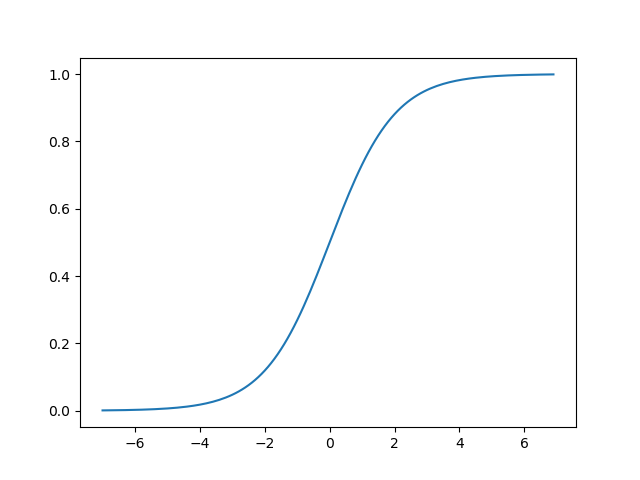
\includegraphics[width=.9\linewidth]{logistic.png}
					\caption{Funzione logistica}
					\label{fig:logistic}
				\end{subfigure}
				\hfill
				\begin{subfigure}[]{.5\textwidth}
					\centering
					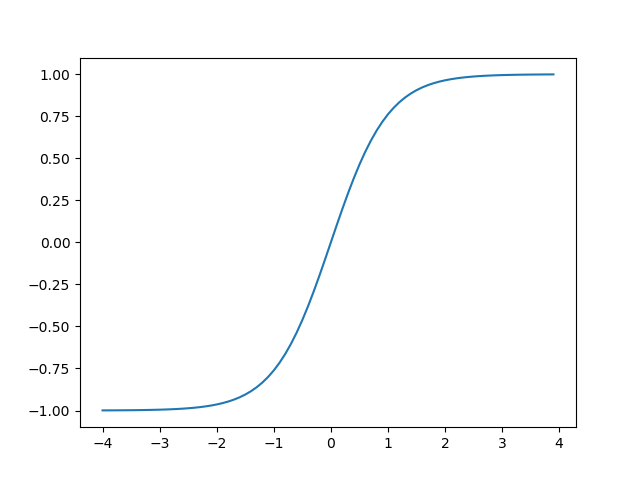
\includegraphics[width=.9\linewidth]{tanh.png}
					\caption{Funzione tangente iperbolica}
					\label{fig:tanh}
				\end{subfigure}
				
				\bigskip  
				
				\begin{subfigure}[]{.5\textwidth}
					\centering
					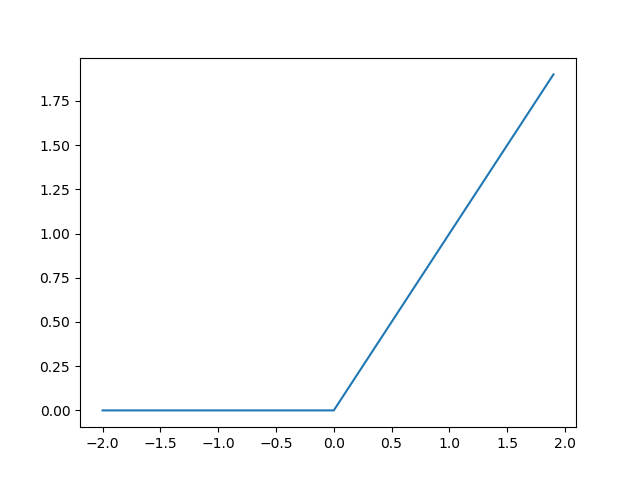
\includegraphics[width=.9\linewidth]{relu.png}
					\caption{Funzione ReLU}
					\label{fig:relu}
				\end{subfigure}
				\hfill
				\begin{subfigure}[]{.5\textwidth}
					\centering
					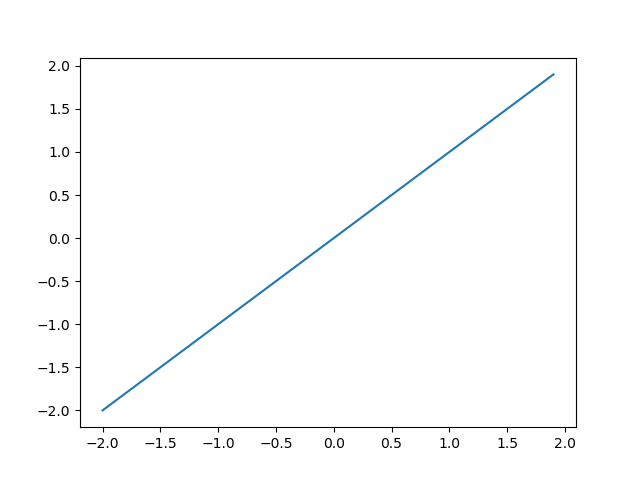
\includegraphics[width=.9\linewidth]{identity.png}
					\caption{Funzione di identità}
					\label{fig:identity}
				\end{subfigure}
				
				\caption{Funzioni di attivazione}
				\label{fig:funzioni di attivazione}
			\end{figure}	
			 	
			 \paragraph{Funzione di uscita} La funzione di uscita di un neurone $j$ calcola i valori che verranno trasmessi agli altri neuroni connessi a $j$. 
			 
			 	Sia $j$ un neurone. La funzione di uscita calcola il valore di output $o_j$ del neurone $j$ in funzione dell'attivazione $a_j$. $$o_j = f_{out}(a_j)$$  
			 	
			 	Anche in questo caso, solitamente la funzione è definita globalmente. Spesso viene usata come funzione di uscita la \textit{funzione di identità}, mandando in output direttamente l'attivazione $a_j$. $$f_{out}(a_j) = a_j, \text{ quindi } o_j = a_j$$
			 	
			 \paragraph{Neurone bias} I valori di soglia $\Theta_{j_1}, \dots, \Theta_{j_n}$ dei neuroni $j_1, \dots, j_n$ possono essere realizzati come pesi di un neurone sempre attivo. Aggiungiamo quindi un neurone \textit{bias} il cui \textit{output} è fisso a 1, connesso ai neuroni $j_1, \dots, j_n$ il cui peso delle connessioni è pari a $-\Theta_{j_1}, \dots, -\Theta_{j_n}$. Questa semplificazione permette di semplificare i conti quando si derivano delle proprietà formali del modello e rendono il codice più efficiente.
			 
			 	\img{Due reti equivalenti, a destra con neurone bias e a sinistra senza. \cite{kriesel}}{0.5}{bias-neuron.png}{bias}
			 	
			 \paragraph{Vettore d'ingresso e vettore di uscita} Le reti neurali che andremo a vedere \textit{(cioè le reti neurali feed-forward)} fanno parte di quella categoria di reti che processano dei dati in input per poi produrre un output. Una rete con $n$ neuroni di ingresso, necessita di un \textbf{vettore d'ingresso} $x = (x_1, x_2, \dots, x_n)$ che gli verrà dato in input e fornisce un \textbf{vettore di uscita} $y = (y_1, y_2, \dots, y_m)$.  
			 	 			 
		\section{Reti neurali feed-forward}
			Esistono diverse topologie di rete, ma noi ci concentreremo sulle \textbf{reti neurali feed-forward} \textit{(o in italiano, reti neurali con flusso in avanti)}. In queste reti, i neuroni sono raggruppati in diversi \textbf{strati}: \textit{uno strato di ingresso, $k$ strati nascosti} e \textit{uno strato di uscita}. In una rete feed-forward ogni neurone ha connessioni dirette solo con lo strato successivo a quelli in cui è contenuto (in direzione dello strato di uscita), evitando così l'esistenza di cicli. Una rete feed-forward in cui ogni neurone è connesso a tutti i neuroni dello strato successivo viene detta rete \textbf{completamente connessa}.

			\paragraph{Percettrone} Un percettrone è una rete feed-forward completamente connessa costituita da uno strato d'ingresso in cui i neuroni di input propagano l'informazione ricevuta \textit{(cioè le funzioni di propagazione, attivazione e uscita del primo strato di neuroni sono la funzione identità)}, seguito da almeno uno strato di pesi addestrabili.
			
			\paragraph{Percettrone a singolo strato} Un percettrone a singolo strato è il percettrone più semplice che si possa fare. Esso è costituito da uno strato di neuroni d'ingresso e uno di uscita. 
				\img{Percettrone a singolo strato con 5 neuroni di ingresso e 3 neuroni di uscita. \cite{kriesel}}{0.5}{slp.png}{slp} 
				
			\paragraph{Separabilità lineare} Siano $X$ e $Y$ due insiemi $\in \mathbb{R}^b$. Essi sono linearmente separabili se e solo se esiste un iperpiano $P$ di $\mathbb{R}^b$ tale che gli elementi di $X$ e $Y$ sono divisi da $P$. 
			
			\begin{figure}
				\begin{subfigure}[]{.5\textwidth}
					\centering
					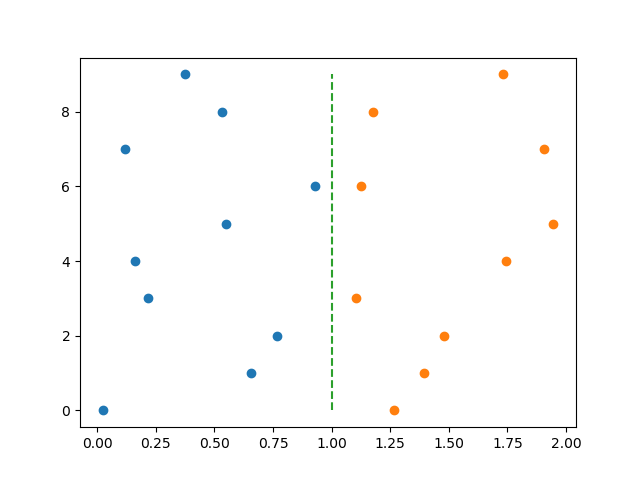
\includegraphics[width=.9\linewidth]{linearly_separable.png}
					\caption{Dati separabili linearmente}
					\label{fig:linearly_separable}
				\end{subfigure}
				\hfill
				\begin{subfigure}[]{.5\textwidth}
					\centering
					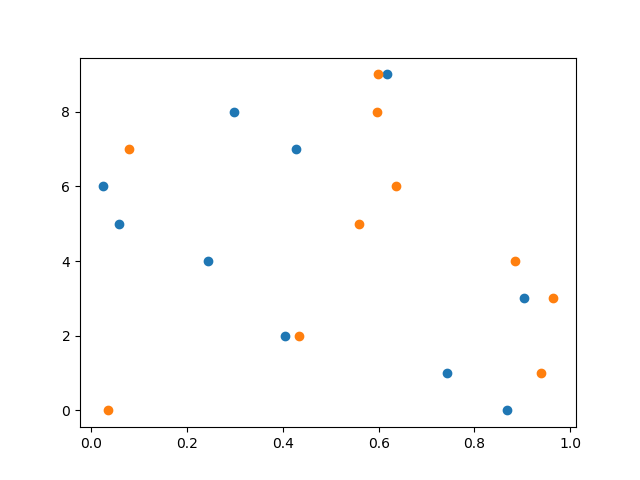
\includegraphics[width=.9\linewidth]{not_linearly_separable.png}
					\caption{Dati \textbf{non} separabili linearmente}
					\label{fig:not_linearly_separable}
				\end{subfigure}
				
				\caption{Separabilità lineare}
			\end{figure}	

				
				 
			\paragraph{Percettrone multistrato} Un percettrone multistrato è una rete feed-forward che ha più di uno strato di pesi addestrabili. M. Minsky e S. Papert nel 1969 dimostrarono in \textit{Perceptrons: an introduction to computational geometry} che i percettroni a singolo strato sono in grado di approssimare solo funzioni che separano i dati \textbf{linearmente}; i percettroni multistrato ci permettono di aggirare questa limitazione. 
				\img{Percettrone multistrato. \cite{kriesel}}{0.5}{nn-feed-forward.png}{feedforward}
		
		\section{Apprendimento di una rete neurale}
			Abbiamo visto la struttura delle reti neurali ma ancora non sappiamo niente su come esse apprendano. Sappiamo che in una rete feed-forward ogni neurone è collegato tramite degli archi pesati a tutti i neuroni dello strato successivo, ma non sappiamo come i pesi vengano inizializzati e in base a cosa vengano modificati. In realtà il processo di apprendimento può essere descritto in pochi passi: 
			\begin{itemize}
				\item dare in input alla nostra rete un vettore d'ingresso $p$ di cui sappiamo l'etichetta,
				\item propagare in avanti l'input attraverso le tre funzioni viste prima, %virgola o punto?
				\item siano $y$ il vettore di uscita ottenuto e $t$ il vettore di uscita desiderato: sottraendo i due vettori otteniamo un \textbf{vettore di errore} $E_p = t - y$,
				\item correggere i pesi con lo scopo di ridurre al minimo $E_p$,
				\item reiterare finchè non si raggiunge un errore soddisfacente.
			\end{itemize}
			Questo è un processo iterativo su due dimensioni. Si itera più volte (finchè non consideriamo l'errore soddisfacente) su tutti i dati. Nonostante la differenza del vettore di errore converga verso un valore basso, questo non ci garantisce che la rete abbia appreso il pattern che c'è dietro ai dati, anzi, potrebbe aver imparato a riprodurre l'output dei dati che gli abbiamo dato in ingresso. Questo fenomeno è chiamato \textbf{overfitting} e per accorgerci di questo problema è buona prassi dividere in due insiemi i dati che usiamo per allenare la rete neurale in: 
			%fondere curva di apprendimento e altro (in monitorare) e aggiungere la parte qua sopra dopo che ci si pone il problema se ha generalizzato
			\begin{itemize}
				\item un insieme di \textbf{training} utilizzato per allenare la rete,
				\item un insieme di \textbf{test} utilizzato per valutare la bontà della rete.
			\end{itemize}
			Una \textit{best practice} è quella di dividere in modo casuale i dati talché siano influenzati il meno possibile da fattori esterni \textit{(per esempio prendere i primi dati in un dataset in cui essi sono ordinati in ordine crescente potrebbe influire negativamente sull'apprendimento)} e solitamente si tiene una proporzione in cui l'insieme di training ha un numero di dati maggiore rispetto all'insieme di validation (almeno 3/4 dei dati totali). 

			\paragraph{Apprendimento online e offline} Oltre alla principale distinzione vista in precedenza tra i tipi di apprendimento (supervisionato e non supervisionato), c'è un'altra distinzione importante sulla frequenza della modifica dei pesi. L'apprendimento può essere: 
				\begin{itemize}
					\item \textbf{Online:} i dati di training vengono inseriti uno a uno, la rete calcola l'errore del singolo dato e modifica i pesi di conseguenza.
					\item \textbf{Offline:} Tutti i dati di training vengono inseriti nella rete insieme, la rete accumula gli errori e modifica i pesi di conseguenza. Ogni lotto di dati viene detto \textbf{batch}, e tutta la procedura di apprendimento dell'intero insieme viene detta \textbf{epoca}.
				\end{itemize}
				Esiste anche una via di mezzo in cui i dati vengono divisi in \textbf{mini-batch}, ovvero sottoinsiemi dell'insieme di training. Dati $h$ dati di training e una dimensione di batch $b$, in ogni epoca i pesi vengono ricalcolati $\lceil h/b \rceil$ volte.
			
			\subsection{Monitorare l'apprendimento di una rete neurale}
				Un modo spesso usato per monitorare l'apprendimento di una rete neurale è quello di tracciare \textbf{curva di apprendimento}. Essa traccia il progresso dell'errore e ci aiuta a capire se la nostra rete stia facendo progressi o meno. Per questo scopo normalizziamo l'errore in modo tale che sia sempre un valore positivo. Il modo più comune è quello di calcolare il valore efficace tra il vettore di uscita desiderato $t$ e il vettore di uscita $y$. 

				Siano $\Omega$ i neuroni di uscita, $O$ l'insieme dei neuroni di uscita e $P$ l'insieme di training. Il valore efficace si calcola nel seguente modo: $$Err_p = \sqrt{\frac{\sum_{\Omega \in O} (t_{\Omega} - y_{\Omega})^2}{|O|}}.$$
				Per quanto riguarda l'apprendimento offline, l'\textbf{errore totale} di un'epoca si calcola nel seguente modo: $$Err = \sum_{p \in P} \frac{Err_p}{|P|}.$$ 
				La curva di apprendimento va tracciata per i due insiemi di training e test, in questo modo possiamo accorgerci se siamo in un caso di overfitting guardando solo l'andamento delle due curve: se la curva di training decresce velocemente mentre quella di test comincia a risalire siamo chiaramente in un caso in cui stiamo perdendo la generalizzazione dei dati che avevamo acquisito, l'ideale sarebbe fermarsi appena prima che la curva di test cominci a risalire (\textbf{early stopping}). Solitamente la curva di training avrà comunque un errore minore rispetto quella di test.

				\begin{figure}
				\begin{subfigure}[]{.5\textwidth}
					\centering
					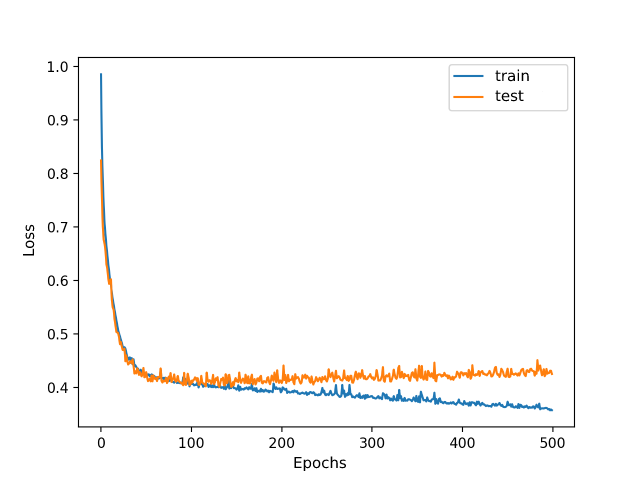
\includegraphics[width=\linewidth]{learning_curve.png}
					\caption{Curva di apprendimento regolare}
					\label{fig:learning_curve}
				\end{subfigure}
				\hfill
				\begin{subfigure}[]{.5\textwidth}
					\centering
					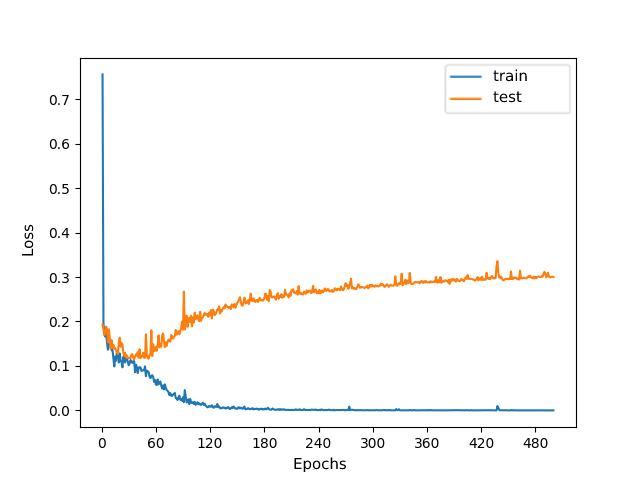
\includegraphics[width=\linewidth]{overfitting.png}
					\caption{Curva di apprendimento con overfitting}
					\label{fig:overfitting}
				\end{subfigure}
				
				\caption{Curve di apprendimento degli insiemi di training e test}
				\label{fig:curve_di_apprendimento}
				\end{figure}
				
			
			\subsection{Discesa del gradiente}
				Ora dovrebbe venire spontaneo chiederci: quando smettiamo di apprendere? Non è una domanda dalla risposta facile, e per capire questo fondamentale passaggio bisogna avere un'idea di cosa sia la discesa del gradiente. È una procedura che viene utilizzata per massimizzare o minimizzare una funzione. Il gradiente è un vettore $g$ definito in ogni punto derivabile di una funzione ed esso punta verso la salita più ripida. Di conseguenza $-g$ punterà verso la discesa più ripida.
				\img{Discesa del gradiente di una funzione a due dimensioni. \cite{kriesel}}{0.5}{gradient_descent_2d.png}{gradient_descent}

				\paragraph{Gradiente} Sia $g$ un gradiente. Allora $g$ è il vettore con $n$ componenti che è definito in ogni punto derivabile di una funzione a $n$ dimensioni $f(x_1, x_2, \dots, x_n)$. L'operatore gradiente è definito come $$g(x_1, x_2, \dots, x_n) = \triangledown f(x_1, x_2, \dots, x_n).$$
					$g$ punta da ogni punto derivabile di $f$ verso la salita più ripida, con una pendenza pari a $|g|$. \cite{kriesel}
				
				\paragraph{Discesa del gradiente} Sia $f$ una funzione a $n$ dimensioni e $s=(s_1, s_2, \dots, s_n)$ il dato punto di partenza. \textbf{Discesa del gradiente} significa andare da $f(s)$ in direzione di $-g$, con passi di dimensione $||g||$ (norma di $g$) verso valori sempre minori di $f$. \cite{kriesel}
				
				\img{Problemi della tecnica della discesa del gradiente \cite{kriesel}}{0.4}{gradient_descent.png}{gradient_descent}
				
				Questa tecnica purtroppo non è priva di problemi, potremmo cadere in diverse \say{trappole} senza accorgercene. Alcuni esempi sono: 
				\begin{itemize}
				 	\item Incagliarsi su un minimo locale non soddisfacente (Figura \ref{gradient_descent}a).
				 	\item Rallentare la ricerca del minimo a causa di un \textit{plateau} (Figura \ref{gradient_descent}b).
				 	\item Trovare un \say{canyon stretto} e continuare ad oscillare a causa dell'elevato contrasto tra i gradienti (Figura \ref{gradient_descent}c).
				 	\item Saltare un buon minimo a causa di una pendenza elevata (Figura \ref{gradient_descent}d).
				 \end{itemize} 
				 
				 
				 \paragraph{Funzione di errore} Ciò che noi vogliamo minimizzare è l'errore totale, ma per come l'abbiamo definito prima non è una funzione, quindi non sarebbe applicabile la discesa del gradiente. L'errore totale cresce o decresce in base a come cambiamo i pesi, quindi possiamo ridefinirlo come una \textbf{funzione di errore} che calcola l'errore normalizzato in funzione dei pesi $$Err : W \rightarrow \mathbb{R}$$ 
				 $$\Delta \omega(i,\Omega) = \nu \cdot o_i \cdot \delta_{\Omega}.$$
			\subsection{Backpropagation}
				
				
	\chapter{Tecniche utilizzate}
		In questo capitolo verrà fatta una panoramica sulle tecniche di \textbf{preprocessing}, \textbf{model selection} e \textbf{over-sampling} utilizzate negli esperimenti svolti. Questo aiuterà a capire con più facilità ciò di cui si parlerà nel capitolo \ref{chap:esperimenti}.
		\section{Preprocessing}
			Nel machine learning, il preprocessing dei dati è uno step facoltativo in cui si trasformano e/o codificano i dati con l'idea di renderli più facili da \say{digerire} da parte del modello di apprendimento. In un dataset, i dati sono rappresentati da delle \textbf{feature}; esse possono acquisire diverse tipologie tra cui: 
			
			\begin{itemize}
				\item \textbf{categoriche:} sono quelle caratteristiche i cui valori fanno parte di un insieme ben definito in cui il numero di valori è solitamente fissato \textit{(ad esempio i valori booleani: true, false; i colori: rosso, verde, blu, ecc...)},
				\item \textbf{numeriche:} sono quelle caratteristiche i cui valori sono rappresentati da numeri (interi o continui) con cui è possibile fare calcoli \textit{(ad esempio i numeri reali, i numeri naturali, ecc...)}.
			\end{itemize}
			Esistono diverse tecniche di preprocessing, ma qui ci concentreremo solo su quelle che useremo durante gli esperimenti.
			
			\subsection{Riduzione della dimensionalità} In un dataset la dimensionalità è il numero di feature presenti. Con riduzione della dimensionalità si intende quell'insieme di tecniche che mirano a ridurre questo valore producendo una versione più compressa dei dati o eliminando delle feature. Queste tecniche vengono spesso utilizzate per visualizzare un insieme di dati in dimensionalità comode per noi umani (solitamente 2 o 3 dimensioni) o per aiutare un modello predittivo ad essere più efficiente e ad ignorare informazioni ridondanti o pressoché inutili che non aiutano particolarmente. 
			
				\subsubsection{Feature selection} La feature selection è quel sottoinsieme di tecniche di riduzione della dimensionalità che include la completa rimozione di alcune feature dall'intero dataset. I modi in cui scegliere quali feature filtrare sono diversi, variano da analisi statistiche \textit{(ad esempio eliminare la feature con varianza minore)} ad analisi sull'accuratezza del modello predittivo. Una buona feature selection, oltre a rendere più veloce la fase di apprendimento da parte del modello, potrebbe aumentarne l'accuratezza.
				
				\subsubsection{Analisi delle componenti principali} L'analisi delle componenti o \textbf{PCA} \textit{(da Principal Component Analysis)} è una tecnica di riduzione della dimensionalità dei dati che punta a ridurre le feature in una loro versione più compressa evidenziandone le componenti principali e massimizzandone la varianza. Il tutto avviene tramite una \textbf{trasformazione lineare} dei dati che vengono proiettati su una dimensione uguale o inferiore.
				\img{Proiezione dei dati da due a una dimensione con PCA \cite{bitsofdna}}{0.3}{pca.jpg}{pca}
				Sia $X$ una matrice con $n$ righe e $m$ colonne in cui ogni riga $x_i$ corrisponde a una misurazione diversa di un esperimento.  Si calcola la media delle righe 
				$$\overline{x}= \frac{1}{n} \sum_{j=1}^n x_j$$ 
				e tramite essa si crea una matrice $\overline{X}$ con $n$ righe in cui ogni riga è $\overline{x}$, si sottraggono le matrici $X$ e $\overline{X}$ ottenendo così una matrice $B$ in cui la media di ogni riga è centrata in zero
				$$B = X - \overline{X},$$
					 e si calcola la matrice di covarianza $C$ delle righe di $B$
					 $$C = B^\top B.$$
					 da $C$ si ricavano gli autovalori $\lambda_1 , \dots, \lambda_m$  e gli autovettori $e_1, \dots, e_n$ che se ordinati in ordine non crescente in una matrice $E$, si ottengono le direzioni degli assi in cui la varianza è massima. Il prodotto $B \cdot E$ trova le coordinate di ogni punto nel nuovo spazio vettoriale e avendo riordinato $E$, se vogliamo ridurre le dimensioni a un numero fissato $k$, allora dovremo eliminare da $E$ le ultime $m-k$ colonne, ottenendo così una matrice con le $k$ componenti principali.  	 
				
				\subsubsection{t-Distributed Stochastic Neighbor Embedding} t-Distributed Stochastic Neighbor Embedding (\textbf{t-SNE}) è una tecnica non lineare di riduzione della dimensionalità. È stato presentato per la prima volta nel 2008 da  L.J.P. van der Maaten e G.E. Hinton nel paper \textit{Visualizing Data using t-SNE} \cite{maaten_hinton}. Tale algoritmo permette la visualizzazione di dati su dimensioni ridotte di varietà topologiche non lineari.
					\img{Visualizzazione di varietà topologiche non lineari con t-SNE utilizando diverse perplessità \cite{sklearn}}{0.35}{tsne.png}{tsne}
				
					\paragraph{Come funziona t-SNE} Per ogni punto $x_i$ si centra una distribuzione gaussiana e si misura la densità di ogni punto $x_j$. Questo ci da un insieme di probabilità $P_{i,j}$ per ogni punto che rappresenta la similarità che ha con gli altri punti. La varianza che determina quanto sia grande il range in cui considerare due punti simili è detta \textbf{perplessità}. Si definisce poi una \textbf{distribuzione di Student} da cui ricaviamo un nuovo insieme di probabilità $Q_{i,j}$ nello spazio dimensionale ridotto. Finalmente si misura la differenza tra le due distribuzioni di probabilità  minimizzando la divergenza di Kullback-Liebler tramite la discesa del gradiente. 
				
					\paragraph{PCA vs t-SNE} 
					
			\subsection{Feature encoding} 
				Abbiamo visto che le feature possono essere categoriche o numeriche, però i modelli di machine learning possono elaborare solo dati numerici. Ovviamente, questo porta a una limitazione per tutti quei dataset in cui sono presenti feature categoriche, ed è qui che entra in gioco la \textbf{feature encoding}. Questo processo serve a trasformare le variabili categoriche in variabile numeriche, e anche qua esistono numerose tecniche. Quando si applica questa procedura bisogna essere cauti a come si procede. Nel rendere numeriche delle variabili categoriche si rischia di creare un ordine inesistente, ma che il modello di apprendimento potrebbe comunque interpretare; ad esempio se dovessimo applicare la tecnica di \textbf{label encoding} su un insieme di colori $\{rosso, blu, verde\}$, essi verrebbero trasformati in $\{0,1,2\}$, e di conseguenza rischieremmo di creare un ordine di importanza per il nostro modello che in realtà esiste: $rosso < blu < verde$.
				
			\subsection{Scalatura dei dati} La scalatura dei dati è una procedura utilizzata per normalizzare i dati presenti in un dataset. Molti modelli di machine learning potrebbero attribuire un valore di importanza maggiore a quelle feature i cui dati variano su ordini di grandezza superiori rispetto ad altri, nonostante non sia sempre ciò che intendiamo trasmettere \textit{(ad esempio se volessimo classificare se un paese è ricco, la popolazione rischierebbe di avere un'influenza maggiore rispetto a un dato come il PIL, che è sicuramente più indicativo)}. Possiamo scalare i dati in diversi modi, qua mostreremo in esempio i metodi presi in considerazione durante gli esperimenti.
			
				\paragraph{Scalatura standard} La scalatura standard viene calcolata per ogni feature $x$ del dataset, centrando la media in zero e dividendo per la deviazione standard. $$z = \frac{x - \overline{x}}{\sigma}.$$
				
				\paragraph{Scalatura min-max} La scalatura min-max viene calcolata per ogni feature $x$ del dataset, scalando i dati in un range compreso tra 0 e 1. $$z = \frac{x - \min(x)}{\max(x) - \min(x)}.$$
			
		\section{Model Selection} 
			Nel machine learning, un iperparametro è un parametro il cui valore è usato per controllare un processo di apprendimento. Alcuni esempi tra quelli che abbiamo visto sono: 
			\begin{itemize}
				\item il numero di neuroni e il numero di strati nascosti in un percettrone multistrato,
				\item le funzioni di ingresso, attivazione e uscita, 
				\item il learning rate,
				\item il numero di epoche.
			\end{itemize}
			Quando si affronta un esperimento in cui si utilizza una rete neurale o più in generale un modello di machine learning, non è quasi mai immediato capire quale sia la scelta migliore degli iperparametri, ed è per questo che esiste la \textbf{model selection}. Essa rappresenta tutte quelle tecniche che ci guidano verso la scelta degli iperparametri una volta forniti i dati. Quando la quantità di dati è elevata solitamente si dividono i dati in tre insiemi: \textbf{train}, \textbf{validation} e \textbf{test}. L'insieme di training viene usato per allenare il modello con le diverse combinazioni di iperparametri, che poi vengono valutati con l'insieme di validation. Una volta trovato il miglior modello, lo si allena nuovamente con i dati di training e validation e lo si testa con l'insieme di test. Se la generalizzazione è simile a quella ottenuta con l'insieme di validation, essa si considera buona. La distribuzione dei dati deve essere la stessa per ogni insieme, altrimenti si rischia di compromettere i risultati. Con un insieme di dati sblilanciato si deve far particolarmente attenzione a questo problema, utilizzando tecniche come l'allocazione ottima di Neyman \textit{(stratified sampling)}. 
			
			\subsection{Cross validation}
				Purtroppo nel mondo reale non sempre si hanno a disposizione un'elevatà quantità di dati, e quindi fare la divisione specificata prima potrebbe pregiudicare la fase di training del nostro modello in quanto avremmo ancora meno dati. 
				
			\subsection{Grid search CV}
	
		\section{Over-sampling}
			\subsection{Synthetic Minority Over-sampling Technique}
		
	\chapter{Esperimenti} \label{chap:esperimenti}
		\section{Dataset} %ricordarsi di scrivere che nel dataset è presente "DATA" ma è stata lasciata fuori in quanto era il campo che discriminava maggiormente, e ragionevolmente ha poco senso.
		\section{Esperimenti di classificazione}
		\section{Reingegnerizzazione dei dati}
		\section{Data augmentation}

	\chapter*{Conclusione}	\addcontentsline{toc}{chapter}{Conclusione}  
	
	\begin{thebibliography}{9}
		\bibitem{kriesel} David Kriesel, 2007, \textit{A Brief Introduction to Neural Networks}, available at \texttt{http://www.dkriesel.com}.

		\bibitem{shwartz} Shai Shalev-Shwartz, Shai Ben-David, 2014, \textit{Understanding Machine Learning: From Theory to Algorithms}, Cambridge University Press.
		
		\bibitem{bitsofdna} Bits of DNA, \texttt{https://liorpachter.wordpress.com/}.
		
		\bibitem{maaten_hinton} Laurens van der Maaten, Geoffrey Hinton, 2008, \textit{Visualizing Data using t-SNE}, Journal of Machine Learning Research 9 2579-2605.
		
		\bibitem{sklearn} Scikit-learn, \texttt{https://scikit-learn.org/}.
		
	\end{thebibliography}
	
\end{document}



